\PassOptionsToPackage{unicode=true}{hyperref} % options for packages loaded elsewhere
\PassOptionsToPackage{hyphens}{url}
\PassOptionsToPackage{dvipsnames,svgnames*,x11names*}{xcolor}
%
\documentclass[paper=a4,justified,a4paper]{tufte-handout}
\usepackage{lmodern}
\usepackage{amssymb,amsmath}
\usepackage{ifxetex,ifluatex}
\usepackage{fixltx2e} % provides \textsubscript
\ifnum 0\ifxetex 1\fi\ifluatex 1\fi=0 % if pdftex
  \usepackage[T1]{fontenc}
  \usepackage[utf8]{inputenc}
  \usepackage{textcomp} % provides euro and other symbols
\else % if luatex or xelatex
  \usepackage{unicode-math}
  \defaultfontfeatures{Ligatures=TeX,Scale=MatchLowercase}
\fi
% use upquote if available, for straight quotes in verbatim environments
\IfFileExists{upquote.sty}{\usepackage{upquote}}{}
% use microtype if available
\IfFileExists{microtype.sty}{%
\usepackage[]{microtype}
\UseMicrotypeSet[protrusion]{basicmath} % disable protrusion for tt fonts
}{}
\IfFileExists{parskip.sty}{%
\usepackage{parskip}
}{% else
\setlength{\parindent}{0pt}
\setlength{\parskip}{6pt plus 2pt minus 1pt}
}
\usepackage{xcolor}
\usepackage{hyperref}
\hypersetup{
            pdftitle={Assignment 7 - Lesson Re-design},
            pdfauthor={Helena Rasche},
            colorlinks=true,
            linkcolor=Maroon,
            filecolor=Maroon,
            citecolor=Blue,
            urlcolor=Blue,
            breaklinks=true}
\urlstyle{same}  % don't use monospace font for urls
\usepackage{longtable,booktabs}
% Fix footnotes in tables (requires footnote package)
\IfFileExists{footnote.sty}{\usepackage{footnote}\makesavenoteenv{longtable}}{}
\setlength{\emergencystretch}{3em}  % prevent overfull lines
\providecommand{\tightlist}{%
  \setlength{\itemsep}{0pt}\setlength{\parskip}{0pt}}
\setcounter{secnumdepth}{0}
% Redefines (sub)paragraphs to behave more like sections
\ifx\paragraph\undefined\else
\let\oldparagraph\paragraph
\renewcommand{\paragraph}[1]{\oldparagraph{#1}\mbox{}}
\fi
\ifx\subparagraph\undefined\else
\let\oldsubparagraph\subparagraph
\renewcommand{\subparagraph}[1]{\oldsubparagraph{#1}\mbox{}}
\fi

% set default figure placement to htbp
\makeatletter
\def\fps@figure{htbp}
\makeatother

\usepackage{pdfpages}

%%%%%%%%%%% Header and Footer %%%%%%%%%%%%%%%%%%
\fancyfoot[CE,CO]{\flushright 
\includegraphics[width=3cm]{../avans.jpg}}
\fancyhead[CE,CO]{\flushleft \smallcaps{\today}}


\title[A7 - Lesson Re-design]{Assignment 7 - Lesson Re-design}
\author{Helena Rasche}
\date{2022-02-07}

\begin{document}
\maketitle
\begin{abstract}
The lesson to be re-designed is Computational Biology, Day 3: De Novo
Genome Assembly, which unfortunately currently experiences poor
coherence between assessment, learning objectives, and learning
activities. This will be improved by taking the solid core of the lesson
and expanding it to further test student's abilities and align with
overall course and program goals.
\end{abstract}
\noindent\rule{5in}{0.4pt}


\hypertarget{the-situation}{%
\section{The situation}\label{the-situation}}

Currently the lesson features the following components:

\begin{longtable}[]{@{}ll@{}}
\toprule
\begin{minipage}[b]{0.31\columnwidth}\raggedright
Aspect\strut
\end{minipage} & \begin{minipage}[b]{0.63\columnwidth}\raggedright
Currently\strut
\end{minipage}\tabularnewline
\midrule
\endhead
\begin{minipage}[t]{0.31\columnwidth}\raggedright
Learning Outcomes\strut
\end{minipage} & \begin{minipage}[t]{0.63\columnwidth}\raggedright
LO1) Compute and interpret a whole genome assembly, LO2) Judge the
quality of a genome assembly.\strut
\end{minipage}\tabularnewline
\begin{minipage}[t]{0.31\columnwidth}\raggedright
Learning Activities\strut
\end{minipage} & \begin{minipage}[t]{0.63\columnwidth}\raggedright
Conda (LO1), Spades (LO1), Quast (LO2), Comparison (LO2)\strut
\end{minipage}\tabularnewline
\begin{minipage}[t]{0.31\columnwidth}\raggedright
Assessment\strut
\end{minipage} & \begin{minipage}[t]{0.63\columnwidth}\raggedright
k-mer exploration (no LOs.)\strut
\end{minipage}\tabularnewline
\bottomrule
\end{longtable}

These are organised in the lecture as:

\begin{itemize}
\tightlist
\item
  An introductory lecture over genome assembly techniques
\item
  Demonstration of assembly
\item
  A hands-on portion where students run the assemblies (LO1)

  \begin{itemize}
  \tightlist
  \item
    Here students run ``Conda'', ``Spades''
  \end{itemize}
\item
  Discussion of genome quality (LO2)

  \begin{itemize}
  \tightlist
  \item
    Here we do ``Quast'', ``Comparison''
  \end{itemize}
\item
  Some formative assessments over their impressions of genome assembly
  qualities
\end{itemize}

\hypertarget{areas-for-improvement}{%
\section{Areas for Improvement}\label{areas-for-improvement}}

This results in very poor coherence currently; the described outcome
``compute and interpret a whole genome assembly'' was marginally
achieved, though the `interpret' step is somewhat lacking. However LO2
is missing very key components:

\begin{itemize}
\tightlist
\item
  There is minimal discussion of quality metrics, and what constitutes a
  good or bad result.
\item
  There are no examples of Good, Mediocre, or Bad
  assemblies\textgreater{}
\item
  While visualisations are available, they are not used.
\item
  The data is assembled twice, with two different settings, which result
  in essentially indistinguishable results (to a trained eye!).
\end{itemize}

And this needs to be significantly improved, there are numerous
low-hanging fruit which can be addressed. Additionally the assessment
portion involves a take-home homework problem set is very theoretical,
incredibly abstract, and related to genome assembly at a very low level.
This hampers students applying knowledge obtained in class to
effectively meet the learning outcomes.

\hypertarget{context-of-the-lesson}{%
\section{Context of the Lesson}\label{context-of-the-lesson}}

This lesson is part of the 3rd year course of BML where students need to
obtain such skills as:

\begin{quote}
\begin{itemize}
\tightlist
\item
  Computer skills: {[}\ldots{}{]} bio-informatics tools, {[}\ldots{}{]}
\item
  Research skills: problem analysis, research questions, {[}\ldots{}{]}
\end{itemize}
\end{quote}

And exists within the Minor Bioinformatica as a 2 EC class, where
students are expected to:

\begin{quote}
{[}\ldots{}{]} you will focus on handling, storing, retrieving and
visualizing massive amounts of biological data. While data generation is
faster than data management, visualization gets more and more important.
{[}\ldots{}{]}
\end{quote}

\hypertarget{improving-lesson-context-coherence}{%
\section{Improving Lesson-Context
Coherence}\label{improving-lesson-context-coherence}}

The above context section gets to the core of the problem.

But here we analyse two relatively small genomes, this should be scaled
up significantly across more samples to truly meet the goals of the
course. This would additionally let us introduce variety of data, good
to bad, and let the students separate those based on their quality
scoring criteria. On top of that, we fail to exercise good visualisation
of the results, and need to introduce that so students have better
comprehension of an incredibly abstract topic.

Students do not get the chance to explore the problem space themselves
and optimise the results, something that would be improved with
integration of more and larger datasets, allowing students to practice
problem analysis and analysing questions applicable to later research.

\hypertarget{content-improvement-plan}{%
\section{Content Improvement Plan}\label{content-improvement-plan}}

The initial part of the lesson covering assembly background is useful
theoretical knowledge for students and should be kept, but maybe
augmented with student activities like ``assembling'' some sentence of
text, to give students an idea of what machines do in the background.
Especially if students are expected to understand k-mers.

\begin{itemize}
\tightlist
\item
  Item 1: Text assembly activity, students split into 3 groups, and get
  to assemble a sentence split with different K-mer values to understand
  consequences.
\end{itemize}

Next, the lesson needs to expand to include a section on evaluation of
genomes by quality metrics as well as a discussion of those major
quality metrics that are used in the field.

\begin{itemize}
\tightlist
\item
  Item 2: (Short) presentation of quality metrics (e.g.~N50, Bandage),
  explanations of their meaning, and then good vs bad results.
\end{itemize}

Finally during the lesson, we will replace the dataset we're using such
that we can have multiple assemblies of various resulting qualities.
Potentially this can be done through a small workflow further exercising
bioinformatics skills they need in the workplaces of their future
employers.

\begin{itemize}
\tightlist
\item
  Item 3: More, smaller genomes of varying quality, tasking students to
  return with a ranking of best to worst assemblies.
\end{itemize}

Lastly the assessments must be augmented, discussing k-mer contributions
is good but not sufficient. This must be expanded to include a further
assembly and quality evaluation, asking them to explore the parameter
space on their own: which parameters resulted in the best assembly? Why
do they think that is the best possible assembly given the data?

\hypertarget{updated-learning-objectives}{%
\section{Updated Learning
Objectives}\label{updated-learning-objectives}}

\begin{itemize}
\tightlist
\item
  Compute multiple whole genome assemblies in such a way to develop big
  data processing skills (Apply+Procedural)
\item
  Learn to evaluate quality metrics so that they can separate good and
  bad assemblies (Analyse+Conceptual, Evaluate+Procedural)
\item
  Visualise assemblies so that they understand presentation of various
  failure modes (Apply+Procedural, Evaluate+Conceptual)
\end{itemize}

\hypertarget{lesson-re-design}{%
\section{Lesson Re-design}\label{lesson-re-design}}

Students will attend this lesson with previous theoretical experience
doing assemblies, this portion is a review for them. They have gone
through the motions of assembly but not done it by hand, nor understood
the intricacies of parameter selection. Students at this stage in their
career are planning to go on to a company or research institute where
they will need to apply these skills to analyse genomic sequences and
help coordinate and design sequencing projects. When those sequencing
experiments occasionally fail for various reasons, they will need to
understand why they failed and how to resolve those issues, be it
parameter exploration or resequencing. This lesson should serve students
well as a very practical lesson delving into comparative analysis which
provides key information for them.

The above described updated learning objectives will allow students to
efficiently approach targeted skills and knowledge as described in the
minor bioinformatic and BML programmes above. This lesson falls near the
end of their curriculum and as such can spend more time focused on an
in-depth understanding of assemblies and their associated failure modes.
The module is titled ``Computational Biology'', which is furthered
through their development of genome assembly skills and computational
scaling of analyses across multiple samples, and visualisation thereof.
This is a task of which they need to become Intermediate practitioners,
in both knowledge and application, within the 2ECs available. By this
point in their career they have already become Novices with assembly and
genomics as topics, letting them now deepen their knowledge and meet
overall Minor Bioinformatica Learning Objectives such as massive data
handling and visualisation.

This lesson's theme is assembly which is supported through several
phases and materials: 1. an assembly activity 2. an initial presentation
on assembly 3. a demonstration portion 4. a hands-on portion where
students work in duos to assemble multiple genomes 5. a subsequent
presentation on quality metrics and visualisation 6. a further hands on
where students apply metrics, visualise, and evaluate all genomes for
quality 7. a group discussion of the results

These will be matched formative assessments in the form of homework
problems which they need to resolve on their own given knowledge from
the lesson. Here they will be tasked with assembling a genome and
exploring the parameter options to optimise the resulting assembly. This
will be complemented with a discussion section where they should explain
why they've chosen those specific parameters to modify. This will aim to
assess their ability to independently answer research questions.

The work forms used in this redesigned lesson will involve lectures,
problem based learning (genome assembly with real world data), group
work in duos (assembly, quality evaluation), and finally group
discussion with peer teaching (as students will explain which one is
better and why to each other.) The in class teaching time is 2.5 hours
which should allow plenty of time for varied work forms to help students
achieve learning goals.

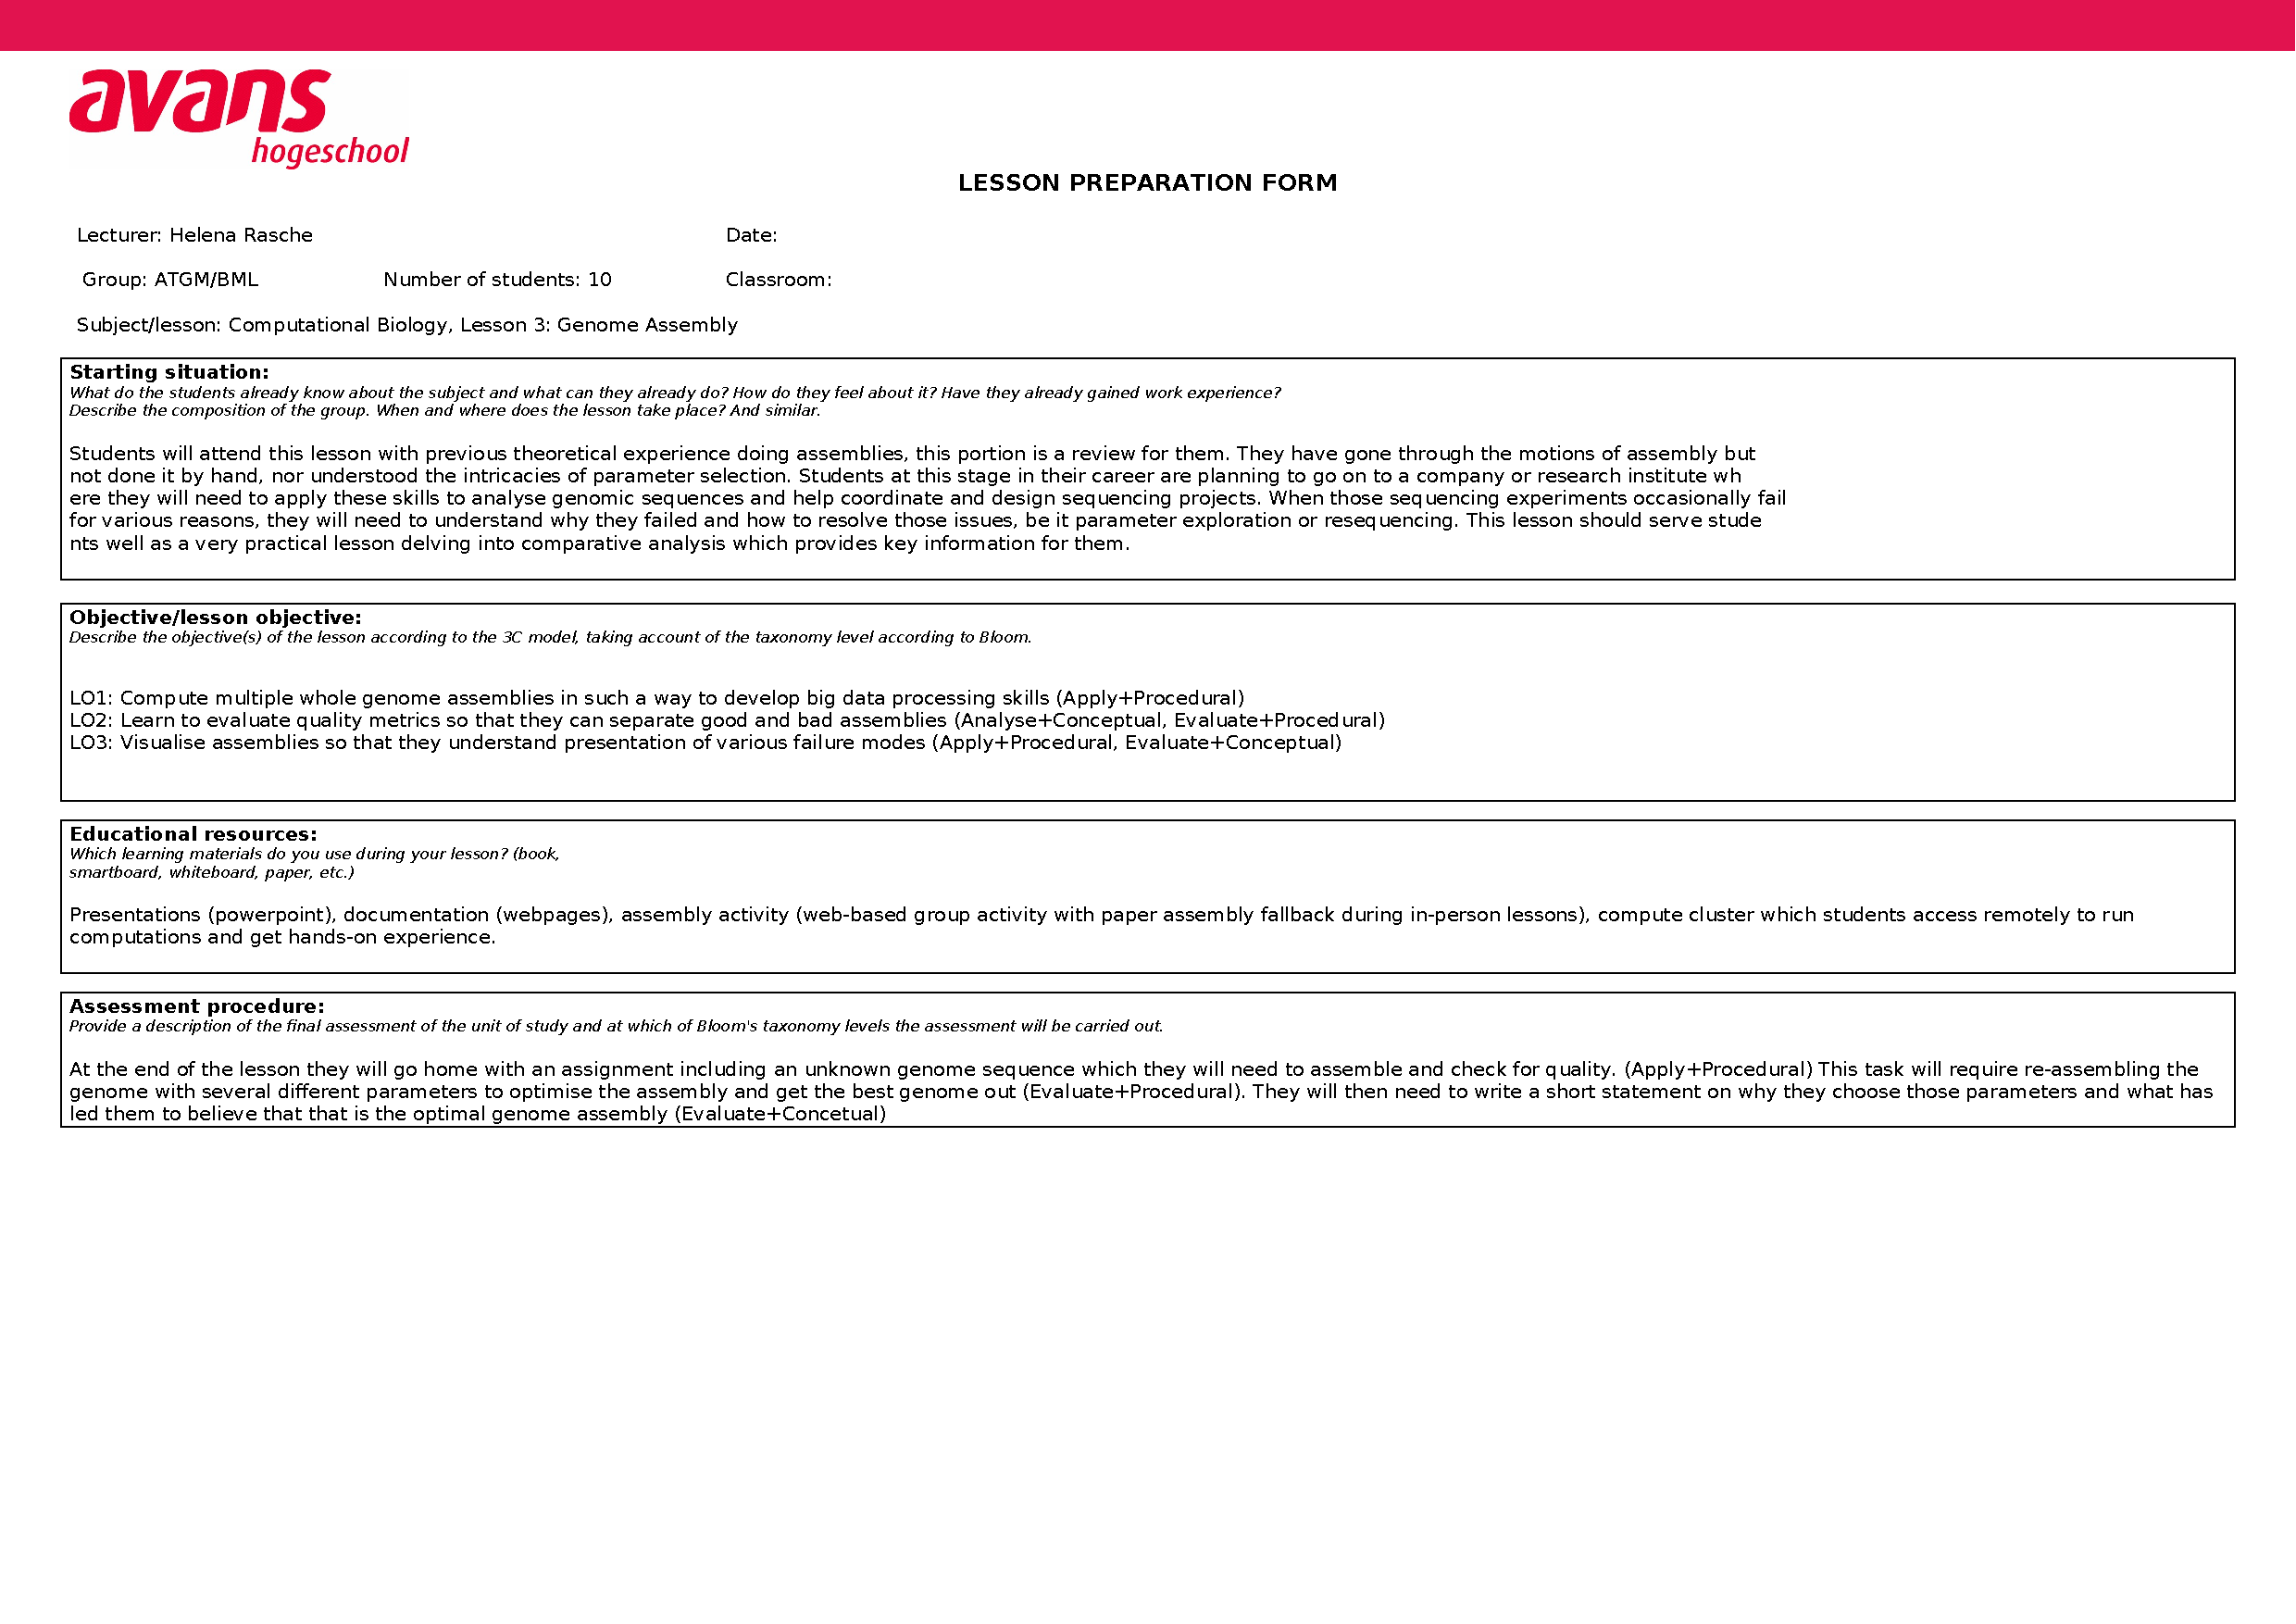
\includepdf[pages=-]{Lesson preparation form v0.pdf}

\end{document}
